% Lists frame
\section{DMC}
\begin{frame}{Wielowymiarowy DMC}
Projekt pętli regulacji z zastosowaniem wielowymiarwego algorytmu DMC:
\begin{itemize}
    \item Wyznaczenie wielowymiarowej odpowiedzi skokowej 
    \item Model w postacji odpowiedźi skokowej
    \item Rozwiązanie problemu optymalizacji
    \item Wyznaczenie wektora optymalnych przyrostów sterowań
\end{itemize}
Wszystkie sygnały sterujące wpływają na sygnały wyjściowe. 
\end{frame}


\begin{frame}{Wielowymiarowy DMC}
Wyznaczenie wielowymiarowej odpowiedzi skokowej:
	\begin{center}
		\begin{figure}[H]
            		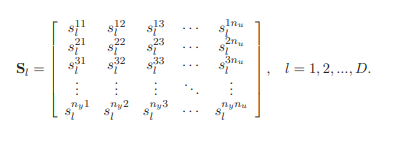
\includegraphics[scale=0.8]{images/wielowymiarowa_odp_DMC.png}
		\end{figure}
	\end{center}
\end{frame}

\begin{frame}{Wielowymiarowy DMC}
Model w postacji odpowiedzi skokowej:
	\begin{center}
		\begin{figure}[H]
            		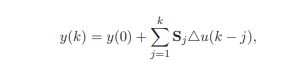
\includegraphics[scale=0.9]{images/model_DMC.png}
		\end{figure}
	\end{center}
\end{frame}

\begin{frame}{Wielowymiarowy DMC}
Rozwiązanie problemu optymalizacji:
	\begin{center}
		\begin{figure}[H]
            		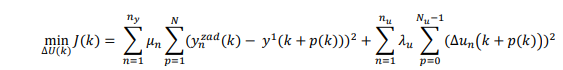
\includegraphics[scale=0.6]{images/cel_DMC.png}
		\end{figure}
	\end{center}
Zależność opisująca wyjścia przewidywane 
\begin{center}
		\begin{figure}[H]
            		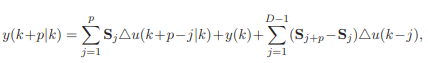
\includegraphics[scale=0.7]{images/wyjscia_DMC.png}
		\end{figure}
	\end{center}
\end{frame}

\begin{frame}{Wielowymiarowy DMC}
Określenie pętli regulacji:
	\begin{center}
		\begin{figure}[H]
            		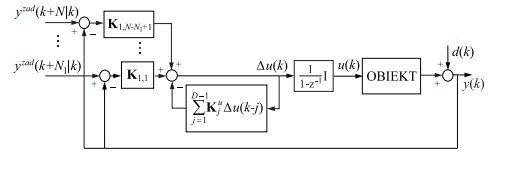
\includegraphics[scale=0.7]{images/SISODMC.png}
          			 \caption{Schemat układu regulacji}
		\end{figure}
	\end{center}
\end{frame}

\begin{frame}{Wielowymiarowy DMC}
Wyniki działania:
	\begin{center}
		\begin{figure}[H]
            		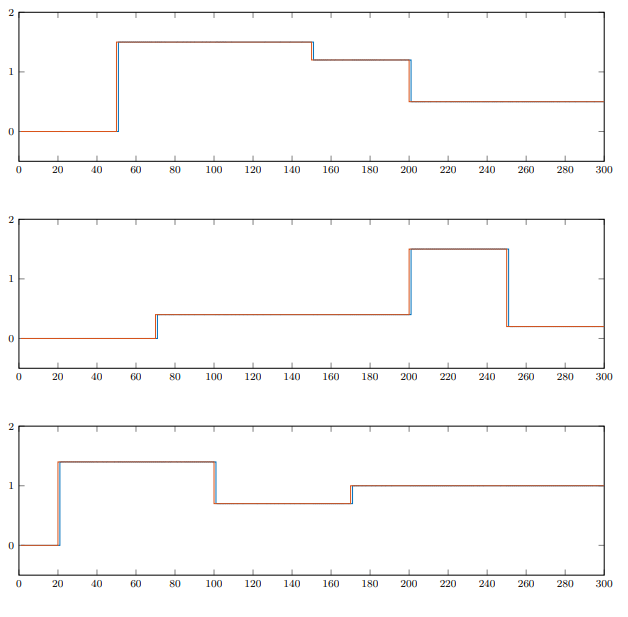
\includegraphics[scale=0.4]{images/wyniki_DMC.png} %%do poprawy jak już będą ładne
          			 \caption{Wyniki wielowymiarowej regulacji z zastosowaniem algorytmu DMC}
		\end{figure}
	\end{center}
\end{frame}
